%%%%%%%%%%%%%%%%%%%%%%%%%%%%%%%%%%%%%%%%%%%%%%%%%%
% Title page template been downloaded from:
% http://www.LaTeXTemplates.com
%%%%%%%%%%%%%%%%%%%%%%%%%%%%%%%%%%%%%%%%%%%%%%%%%%

\documentclass[a4paper]{article}
\RequirePackage[utf8]{inputenc}
\usepackage[portuguese]{babel}
\usepackage{listings}
\usepackage{color}
\usepackage{graphicx}
\usepackage{hyperref}

\definecolor{dkgreen}{rgb}{0,0.6,0}
\definecolor{gray}{rgb}{0.5,0.5,0.5}
\definecolor{mauve}{rgb}{0.58,0,0.82}

\lstset{frame=tb,
  language=Java,
  aboveskip=3mm,
  belowskip=3mm,
  showstringspaces=false,
  columns=flexible,
  basicstyle={\small\ttfamily},
  numbers=none,
  numberstyle=\tiny\color{gray},
  keywordstyle=\color{blue},
  commentstyle=\color{dkgreen},
  stringstyle=\color{mauve},
  breaklines=true,
  breakatwhitespace=true,
  tabsize=3,
  literate=
  {á}{{\'a}}1 {é}{{\'e}}1 {í}{{\'i}}1 {ó}{{\'o}}1 {ú}{{\'u}}1
  {Á}{{\'A}}1 {É}{{\'E}}1 {Í}{{\'I}}1 {Ó}{{\'O}}1 {Ú}{{\'U}}1
  {à}{{\`a}}1 {è}{{\'e}}1 {ì}{{\`i}}1 {ò}{{\`o}}1 {ù}{{\`u}}1
  {À}{{\`A}}1 {È}{{\'E}}1 {Ì}{{\`I}}1 {Ò}{{\`O}}1 {Ù}{{\`U}}1
  {ä}{{\"a}}1 {ë}{{\"e}}1 {ï}{{\"i}}1 {ö}{{\"o}}1 {ü}{{\"u}}1
  {Ä}{{\"A}}1 {Ë}{{\"E}}1 {Ï}{{\"I}}1 {Ö}{{\"O}}1 {Ü}{{\"U}}1
  {â}{{\^a}}1 {ê}{{\^e}}1 {î}{{\^i}}1 {ô}{{\^o}}1 {û}{{\^u}}1
  {Â}{{\^A}}1 {Ê}{{\^E}}1 {Î}{{\^I}}1 {Ô}{{\^O}}1 {Û}{{\^U}}1
  {œ}{{\oe}}1 {Œ}{{\OE}}1 {æ}{{\ae}}1 {Æ}{{\AE}}1 {ß}{{\ss}}1
  {ç}{{\c c}}1 {Ç}{{\c C}}1 {ø}{{\o}}1 {å}{{\r a}}1 {Å}{{\r A}}1
  {€}{{\EUR}}1 {£}{{\pounds}}1
}

\begin{document}

\begin{titlepage}

\newcommand{\HRule}{\rule{\linewidth}{0.5mm}} % Defines a new command for the horizontal lines, change thickness here

\center % Center everything on the page
 
%----------------------------------------------------------------------------------------
%	HEADING SECTIONS
%----------------------------------------------------------------------------------------

\textsc{\LARGE Instituto Superior de Engenharia de Lisboa}\\[1.5cm] % Name of your university/college
\textsc{\Large Sistemas Distribuídos}\\[0.5cm] % Major heading such as course name

%----------------------------------------------------------------------------------------
%	TITLE SECTION
%----------------------------------------------------------------------------------------

\HRule \\[0.4cm]
{ \huge \bfseries Relatório de Trabalho}\\[0.4cm] % Title of your document
{ \Large \bfseries Brokering System (Série 1)}\\
\HRule \\[1.5cm]
 
%----------------------------------------------------------------------------------------
%	AUTHOR SECTION
%----------------------------------------------------------------------------------------

\begin{minipage}{0.4\textwidth}
\begin{flushleft} \large
\emph{Grupo G03D:}\\
32632 Pedro \textsc{Pedroso} \
33404 Ricardo \textsc{Mata} \\
33724 David \textsc{Raposo} \\

\
\end{flushleft}
\end{minipage}
~
\begin{minipage}{0.4\textwidth}
\begin{flushright} \large
\emph{Para:} \\
Engº Luís \textsc{Assunção} \\
\end{flushright}
\end{minipage}\\[4cm]

%----------------------------------------------------------------------------------------
%	DATE SECTION
%----------------------------------------------------------------------------------------
{\large \today}\\[3cm] % Date, change the \today to a set date if you want to be precise

\vfill % Fill the rest of the page with whitespace

\end{titlepage}

%----------------------------------------------------------------------------------------
%	ÍNDICE
%----------------------------------------------------------------------------------------

\newpage
\thispagestyle{empty} %Remove a númeração da página

\tableofcontents

%----------------------------------------------------------------------------------------
%	BODY
%----------------------------------------------------------------------------------------
\newpage
\setcounter{page}{1} %começa a contar as páginas apartir do 1

\section{Introdução}

O primeiro trabalho desta cadeira pede que desenvolvamos um sistema de brokering entre clientes e trabalhadores, sem que estes se conheçam. Serve o presente relatório para
explicar a nossa implementação e para discutir as nossas soluções.

\section{Arquitetura}

A solução tem 3 intervenientes distintos. Um cliente que pretende que sejam realizadas tarefas remotamente, um (ou mais) serviço de execução de trabalhos que irá executar trabalhos submetidos pelo cliente, e um intermediário que irá delegar trabalhos aos serviços de execução. A partir deste ponto passaremos a referirmo-nos ao intermediário como \emph{broker} e aos serviços de execução como \emph{workers} ou \emph{worker}.

O cliente pretende que alguém lhe faça um trabalho. Para isso envia um pedido ao \emph{broker} a dizer qual o trabalho que pretende que seja executado. O \emph{broker} decide então qual o \emph{worker} mais adequado para executar essa tarefa, e envia-lhe o pedido do cliente. Assim que seja possível o worker inicia a execução do trabalho, e assim que o trabalho estiver concluído, notifica o cliente e o broker de que o trabalho foi concluído.


\medskip
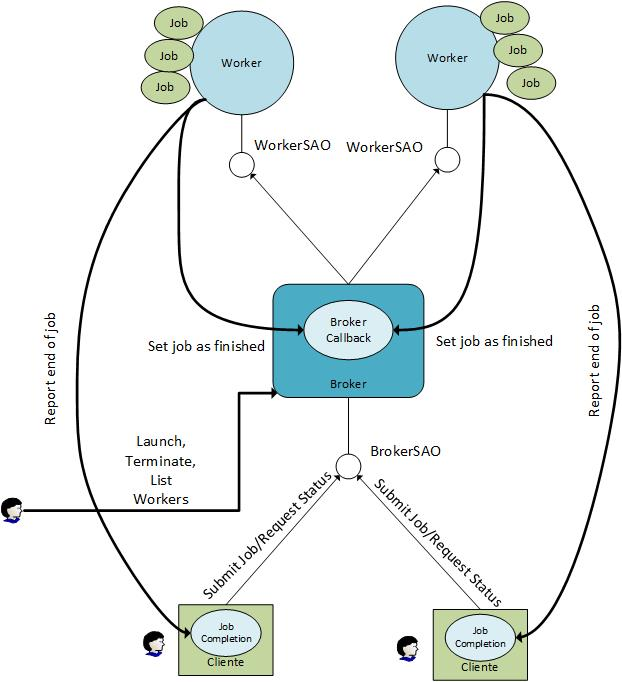
\includegraphics[height=10cm]{arquitectura}


\section{Estruturas}

\subsection{Armazenamento de dados}
\textbf{DataManager:}

O data manager é a class que é usada para armazenamento e manipulação de dados relativos ao broker.

\begin{description}
	\item[JobWrapper:]\hfill
	
	\emph{Class} de armazenamento de informação relativa ao \emph{Job}. Contém:
		\begin{description}
					\item[j:]
					Objecto job com informação para iniciar o processo (id do job,nome do processo, 		ficheiro de input, ficheiro de output e \emph{proxy} para a chamada final ao cliente para sinalizar o fim do trabalho).
					\item[status:]
					\emph{Status} que o job tem (\emph{Queued}, \emph{Running},\emph{Finished}).
			\end{description}
	
	\item[WorkerWrapper:]\hfill
	
	\emph{Class} de armazenamento de informação relativa ao \emph{worker}. Contém:
		\begin{description}
			\item[workerProxy:] \emph{Proxy} para comunicação com o \emph{worker}.
			\item[currentJobs:] Número de trabalhos que o \emph{worker} está a processar de momento.
			\item[dictJobs:] Dicionário com todos os \emph{jobs} que o worker está a processar de momento.
			\item[port:]\emph{Port} associado ao \emph{worker}.
		\end{description}
			
\end{description}

\medskip	
Esta informação é guardada em duas estruturas
		\begin{description}
		\item[\emph{jobDict}:] Dicionário onde a chave é o \emph{id} e o \emph{value} é um objeto \emph{JobWrapper}. Esta estrutura é usada para guardar o progresso dos \emph{jobs} para eventual consulta pelo cliente.
		\item[\emph{workerDict}:] Dicionário onde a chave é o \emph{port} do \emph{worker} e a chave é um \emph{WorkerWrapper}. É usado para associar trabalhos aos respetivos \emph{workers}. Em caso de um \emph{worker} falhar, podemos ressubmeter os trabalhos para outro \emph{worker}.

	\end{description}

\subsection{\emph{Interfaces}}

\textbf{IWorkerSAO:}
	Esta interface disponibiliza os serviços do \emph{worker} para o \emph{broker}: Submissão de \emph{Jobs}, fecho do próprio \emph{worker}, \emph{ping} e requisição do número de \emph{Jobs} a processar de momento. Visto o \emph{worker} abstrair os clientes e o \emph{broker} da execução de trabalhos, estes desconhecem o tempo de execução dos trabalhos, de forma a que o \emph{worker} pode ficar bastante tempo a processar. Os acessos aos objetos dos \emph{workers} também vão ser feitos por uma só entidade, o \emph{broker}, o que nos levou a implementar a interface como \emph{Singlecall} em vez de \emph{Singleton}, pois só vai existir uma instância por \emph{worker} com tempo de vida definido pelo \emph{broker}.

\textbf{IBrokerSAO:}
	Utilizado para os clientes fazerem submissão de \emph{Jobs} ou para verificar o seu estado. Este objeto disponibiliza serviços do \emph{broker} e é acedido por cada cliente que queira fazer um \emph{Job}. Como o \emph{broker} é uma entidade central que pretende delegar os trabalhos aos \emph{workers}, faz sentido que estado das suas estruturas de dados seja visível aos clientes que lhe acedam, por isso implementámos o \emph{broker} como \emph{singleton}.

\section{Implementação}

Configurámos cada uma das partes para se ligarem a uma porta \emph{TCP} como um \emph{Well Known Type}. Isto permite que cada uma das partes consiga comunicar entre si. Esta configuração define os \emph{end-points} onde cada parte irá aceder para poder comunicar com outras partes, e o tipo de canal que é usado para a comunicação.

O cliente regista o \emph{Well Known Type} do \emph{broker} à interface partilhada. Isto permite criar uma interface de comunicação onde cada acesso feito pelo cliente vai ser tratado não localmente, mas pelo \emph{broker}. Um pedido de trabalho é então enviado ao \emph{broker} através dessa interface, e para o pedido de trabalho é criada uma instância do tipo \emph{Job}. Este tipo tem a seguinte informação:
\begin{itemize}
\item O nome do trabalho que se quer executar.
\item Os nomes dos ficheiros input e output.
\item O identificador do trabalho que é dado pelo \emph{broker}, para pedidos de estado.
\item Uma interface para que o \emph{worker} possa avisar diretamente o cliente da conclusão do trabalho.
\end{itemize}

A existência da interface de comunicação para o worker torna este tipo num \emph{proxy}. Isto requer um cuidado extra na configuração dos canais de comunicação (o canal tem de ser configurado como "`\emph{full}"' para que a comunicação seja delegada pelo \emph{broker}). É também de notar que esta solução foi implementada tendo em conta que os \emph{workers} vão estar na mesma máquina que o broker e o cliente (apesar de se simular um ambiente remoto), de forma a que uma solução completamente remota iria necessitar de outra abordagem na passagem de parâmetros/receção de resultados entre o cliente e os \emph{workers}.

Quando o objeto chega ao broker é colocado num mapa de jobs. Este mapa contém informação sobre os \emph{jobs} submetidos para que seja possível ressubmetê-los caso haja necessidade de tal.

\subsection{Modo Automático}
\subsubsection{Adição de workers}
A adição de \emph{workers} em modo automático segue um só critério. Se houver demasiados \emph{Jobs} num \emph{worker}(definido pela variável \emph{NUMBER\_OF\_MAX\_SLOTS\_FOR\_WORKER}) no momento da submissão de um novo \emph{Job}, o \emph{broker} irá criar um novo \emph{worker}.

\subsubsection{Remoção de workers}
A remoção automática é feita segundo o seguinte critério: se houver mais do que um \emph{worker} sem trabalhos, então um deles será removido. Esta verificação acontece sempre que um \emph{Job} seja retirado do \emph{worker}.

\subsection{Modo Manual}
\subsubsection{Adição de workers}
A adição de \emph{workers} é feita simplesmente ao adicionar mais um \emph{worker} ao dicionário de \emph{workers} disponíveis. Durante a atribuição de \emph{Jobs} é escolhido o \emph{worker} com menos trabalhos de momento.

\subsubsection{Remoção de workers}
A remoção de \emph{workers} é feita ao remover um dos \emph{workers} disponiveis do dicionário e caso ainda haja \emph{Jobs} nos \emph{workers}, estes serão resubmetidos a outros \emph{workers}.
Esta remoção é feita utilizando a porta do \emph{worker} como identificação.

\subsubsection{Listagem de \emph{workers}}
É possível listar os \emph{workers} a trabalhar de momento, visualizando a porta onde estão configurados.

\subsection{Configuração dos objectos remotos}
A configuração dos objetos remotos(\emph{BrokerSAO} e \emph{WorkerSAO}) é realizada através de ficheiros de configuração. O ficheiro de configuração do \emph{BrokerSAO} contém o tipo de ligação, a porta da ligação, o nome do \emph{well-known object} e a porta base usada para a criação dos ficheiros de configuração dos \emph{workers}.
Os ficheiros de configuração do \emph{worker} são criados pelo \emph{broker} localmente, que envia o caminho relativo a cada \emph{worker} para este utilizar na sua configuração. A porta a utilizar por cada \emph{worker} é escolhida incrementando a porta base que está presente no ficheiro de configuração do \emph{broker}.


\textbf{Limitação:} Estamos a admitir que os \emph{workers} estão a trabalhar na mesma máquina, assim podemos passar só o caminho dos ficheiros de configuração para os \emph{workers}. No caso dos \emph{workers} estarem a trabalhar em máquinas diferentes, seria necessário passar os parãmetros e seria o próprio \emph{worker} a fazer a sua configuração localmente.


\subsection{Estado do \emph{Job}}
A nossa aplicação atualiza e guarda o estado de cada \emph{Job} ao longo do seu percurso. Estes estados refletem o estado do \emph{job}: quando o \emph{Job} é submetido tem o estado \emph{QUEUED}, quando é enviado para o \emph{worker} tem o estado \emph{RUNNING}, e finalmente quando acaba tem o estado \emph{FINISHED}. 
Estas atualizações são feitas pelo \emph{broker} sendo a ultima feita pelo \emph{worker} que, ao terminar o trabalho, notifica através do \emph{proxy BrokerCallback} qual o \emph{Job} que acabou.
O cliente pode a qualquer momento fazer uma verificação do estado do \emph{Job} através da interface partilhada \emph{IBrokerSAO}.

\textbf{Limitação:} Um cliente pode saber o estado de um Job que não tenha sido ele próprio a criar. Prevenir esta situação implicava verificações adicionais e identificação de cada cliente que iria criar mais \emph{stress} sobre o \emph{broker} e isto não era o objetivo deste trabalho.


\subsection{Suporte e deteção de falhas}

A deteção de falhas de um \emph{worker} ocorre quando há uma tentativa de ligação através do \emph{WorkerSAO} e ocorre uma \emph{socket exception}. Estas deteções são feitas na atribuição de um trabalho ou na verificação de estado do trabalho. Na verificação, como temos os estados do trabalho guardados no \emph{broker} não necessitando portanto fazer uma ligação com o \emph{worker}, fazemos um \emph{ping} ao \emph{worker} associado para verificar a ligação.

No caso de um \emph{worker} falhar, os trabalhos naquele momento a ser processados vão ser perdidos. Detetamos esta situação quando uma tentativa de acesso a um \emph{proxy} resulta numa \emph{Socket Exception}. Nesta situação, o \emph{broker} vai procurar em \emph{workerDict} os \emph{Jobs} associados a este \emph{worker} e vai ressubmetê-los a outros \emph{workers} que estejam activos.	
	
\end{document}